# -*- mode: snippet -*-
\documentclass[12pt, letterpaper]{report}
\usepackage[utf8]{inputenc}
\usepackage[T1]{fontenc}
\usepackage[a4paper,left=2cm,right=2cm,top=2cm,bottom=2cm]{geometry}
\usepackage{booktabs}
\usepackage[french]{babel}
\usepackage{libertine}
\usepackage[pdftex]{graphicx}
\usepackage{csquotes}
\usepackage{url}
\usepackage{hyperref}
\hypersetup{colorlinks=true,linkcolor=black}


\setlength{\parskip}{1em}
\setlength{\parindent}{0em}
\newcommand{\hsp}{\hspace{20pt}}
\newcommand{\HRule}{\rule{\linewidth}{0.5mm}}

\begin{document}
\begin{titlepage}
  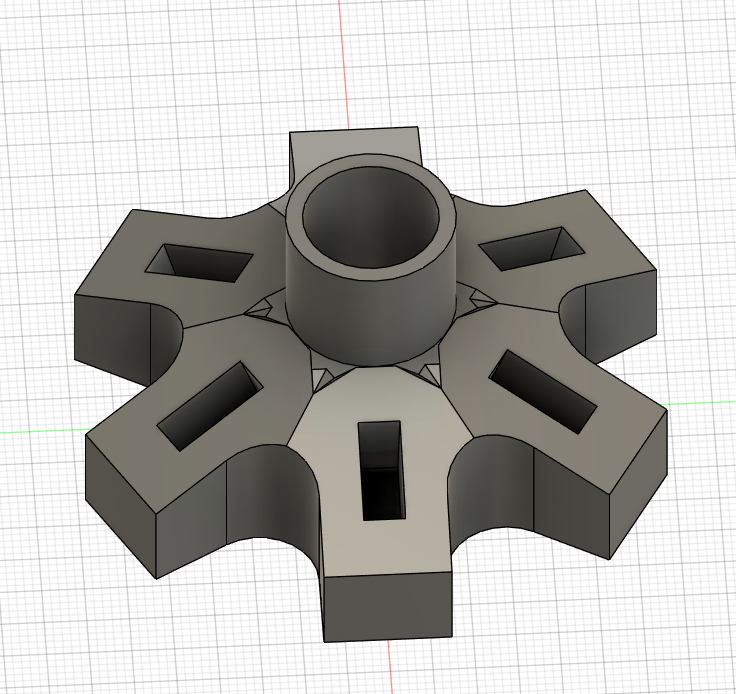
\includegraphics[scale=0.7]{IMG1.JPG}
  \begin{sffamily}
    \begin{center}


      \textsc{\LARGE Henallux - Institut d'enseignement supérieur de Namur}\[2cm]

        \textsc{\Large Laboratoire de sciences appliquées à l'informatique}\[1.5cm]

          \HRule \[0.4cm]
            \huge \bfseries {Laboratoire \#01 - Analyse de signaux \[0.4cm]}
              \HRule \[2cm]

                \begin{minipage}{0.4\textwidth}
                  \begin{flushleft} \large
                    Schoonjans \textsc{Ludovic}\
                    Vanderbeken  \textsc{Mathias}\
                    Dubois  \textsc{Aaron}\
                    Combette  \textsc{Nathan}\
                  \end{flushleft}
                \end{minipage}
                \begin{minipage}{0.4\textwidth}
                  \begin{flushright} \large
                    \emph{Professeur :} \textsc{Guillerme Duvillié}\
                    \emph{Groupe :} \textsc{Les coléoptères \du frigos}\
                  \end{flushright}
                \end{minipage}

                \vfill

                \large 18 Avril 2023
    \end{center}
  \end{sffamily}
\end{titlepage}

\renewcommand*\contentsname{Table des matières}
\tableofcontents

\chapter{}

\chapter{}

\begin{itemize}
\item
\item
\item
\item
\end{itemize}

\bigskip

\chapter{}



\chapter{}

\begin{center}
  \includegraphics[trim={75cm 0 15cm 0},clip,scale=0.1]{Figure1.jpg}
  \includegraphics[trim={25cm 0 55cm 0},clip,scale=0.1]{Figure3.jpg}
  \newline
  \includegraphics[trim={10cm 50cm 0 60cm},clip,scale=0.12,angle=90,origin=c]{Figure5.jpg}
\end{center}

\chapter{Conclusion}

\chapter{Bibliographie}

$[Fig.2.1]$ {https://m.media-amazon.com/images/I/71xb7p6G5lL.\_SX522\_.jpg}

$[1]$ \textsc{Wikipédia}, \emph{Loi d'Ohm}, \newline
{https://fr.wikipedia.org/wiki/Loi\_d\%27Ohm},\quad consulté le 03/04/2023 à 14h43.
\smallskip

$[2]$ \textsc{Wikipédia}, \emph{Décibel}, \newline
{https://fr.wikipedia.org/wiki/Décibel},\quad consulté le 03/04/2023 à 14h02.
\smallskip

$[3]$ \textsc{Wikipédia}, \emph{Énergie électrique},\newline
{https://fr.wikipedia.org/wiki/Énergie\_électrique},\quad consulté le 03/04/2023 à 14h47.

\end{document}
